\section{UC02 - Visualizzazione lista aree}\label{uc:02}

\paragraph{Intenzione in contesto} L'attore primario vuole vedere una lista delle varie aree di illuminazione ed il loro stato.

\paragraph{Attore primario} L'attore primario sono l'utente gestore e manutentore.

\paragraph{Precondizioni} L'attore primario è autenticato ed autorizzato dal sistema.

\paragraph{Postcondizioni} L'attore primario vede la lista delle aree.

\paragraph{Scenario principale}

\begin{enumerate}
    \item L'utente richiede la visualizzazione della lista delle aree;
    \item il sistema fornisce la lista delle aree presenti nel sistema.
\end{enumerate}

\begin{figure}[h]
    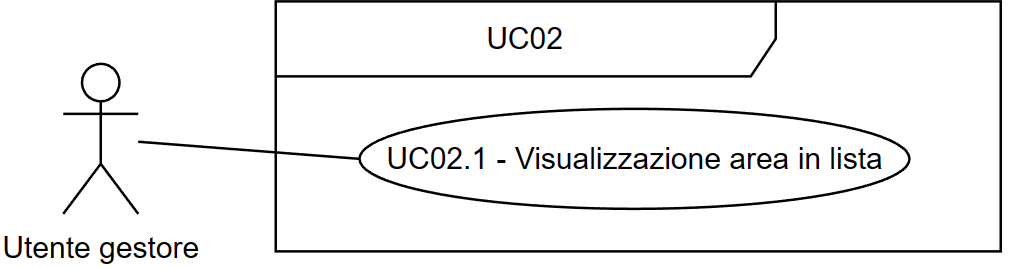
\includegraphics[width=\textwidth]{contenuti/img/casi_uso_grafici-uc02.png}
    \caption{Dettaglio dell'UC02}
    \label{fig:uc02}
\end{figure}

\subsection{UC02.1 Visualizzazione lampioni in area}
\paragraph{Intenzione in contesto} L'attore primario vuole visualizzare una singola area.

\paragraph{Attore primario} L'attore primario è l'utente gestore.
\paragraph{Precondizioni} L'attore primario è riconosciuto ed autorizzato dal sistema.
\paragraph{Postcondizioni} L'attore primario visualizza la singola area desiderata.

\paragraph{Scenario principale}
\begin{enumerate}
    \item L'utente richiede di visualizzare una singola area;
    \item l'utente visualizza la singola area desiderata.
\end{enumerate}

\begin{figure}[h]
    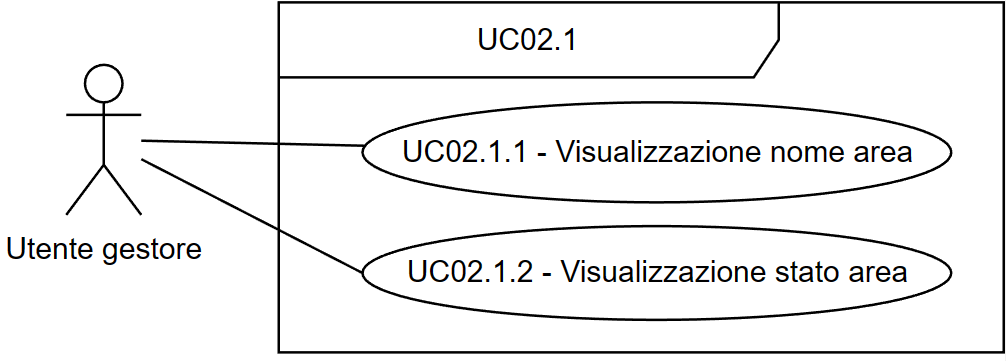
\includegraphics[width=\textwidth]{contenuti/img/casi_uso_grafici-uc02.1.png}
    \caption{Dettaglio dell'UC02.1}
    \label{fig:uc02.1}
\end{figure}

\subsection{UC02.1.1 - Visualizzazione nome area}\label{uc:02.1.1}

\paragraph{Intenzione in contesto} L'attore primario vuole visualizzare il nome dell'area.
\paragraph{Attore primario} L'attore primario è o l'utente gestore manutentore.
\paragraph{Precondizioni}  L'attore primario è autenticato ed autorizzato dal sistema.
\paragraph{Post-condizioni} L'attore primario visualizza il nome dell'area.
\paragraph{Scenario principale}
\begin{enumerate}
    \item L'attore primario richiede al sistema di visualizzare il nome dell'area;
    \item il nome dell'area è stato visualizzato.
\end{enumerate}

\subsection{UC02.1.2 - Visualizzazione stato area}\label{uc:02.1.2}

\paragraph{Intenzione in contesto} L'attore primario vuole visualizzare lo stato dell'area.
\paragraph{Attore primario} L'attore primario è o l'utente gestore manutentore.
\paragraph{Precondizioni}  L'attore primario è autenticato ed autorizzato dal sistema.
\paragraph{Post-condizioni} L'attore primario visualizza lo stato dell'area.
\paragraph{Scenario principale}
\begin{enumerate}
    \item L'attore primario richiede al sistema di visualizzare lo stato dell'area;
    \item lo stato dell'area è stato visualizzato.
\end{enumerate}